% Created 2021-01-12 Tue 21:13
% Intended LaTeX compiler: pdflatex
\documentclass[presentation]{beamer}
\usepackage[utf8]{inputenc}
\usepackage[T1]{fontenc}
\usepackage{graphicx}
\usepackage{hyperref}
\usepackage{multicol}
\usepackage{listings}
\usepackage{enumitem}
\usepackage{minted}
\usetheme{Madrid}
\setbeamertemplate{items}[circle]
\author{Scott Mora}
\date{03-2021}
\title{Tiny Idris Program Synthesis}
\hypersetup{
 pdfauthor={Scott Mora},
 pdftitle={Tiny Idris Program Synthesis},
 pdfcreator={Emacs 27.1 (Org mode 9.3)}, 
 pdflang={English}}
\begin{document}

\maketitle

\begin{frame}[fragile]{Introduction}
  \begin{itemize}
  \item Introduce Functional programs and the TinyIdris system.\\
  \item Project aim \\
  \item Related work \\
  \item Implementation \\
  \item Evaluation \\
  \end{itemize}
\end{frame}  

\begin{frame}[fragile]{Functional Programming}
  \begin{itemize}
  \item Defines the structure of data. \hspace{12em}
\includegraphics[scale=0.3]{Resource/lam.png}\\
  \item Functions transform data by inspecting the structure, and deciding how to proceed.\\
  \item Abstractions lead to concise code and encourages reuse. \\
  \item Similar structures can lead to repetitive code.\\
  \item Repetitive boilerplate can be tedious and lead to simple errors.\\
  \end{itemize}
\end{frame}  

\begin{frame}[fragile]{TinyIdris}
  \begin{itemize}
  \item Tiny Idris is a dependently typed functional language.
  \item Not compiled, runs as an evaluator.
    \begin{block}{}
      \begin{figure} 
        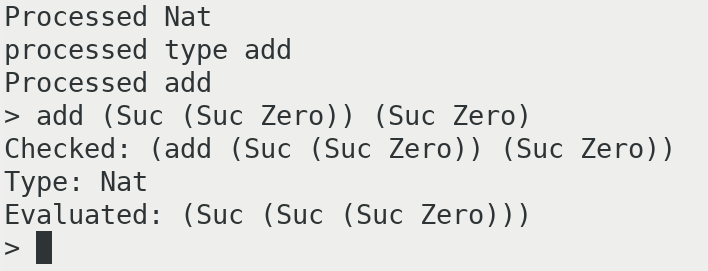
\includegraphics[scale=0.4]{./Resource/addEval.png}
      \end{figure}
    \end{block}
  \end{itemize}
\end{frame}

\begin{frame}[fragile]{Project Aim}
  \begin{itemize}
    \item Extend the TinyIdris system with program synthesis functionality.\\
    \item Constructing a function definition from a type signature, local
          environment and global context.
  \end{itemize}
\end{frame}

\begin{frame}[fragile]{Specialised Systems}
\begin{center}
  
\includegraphics[scale=0.2]{Resource/synquid-logo.png}
  
\includegraphics[scale=0.2]{Resource/resyn-logo.png}
\end{center}
  \begin{itemize}
  \item Specialised tools such as Leon, Myth, Synquid, ReSyn.
  \item No use of available type information initially, use general constraint solving approach.
  \item Utilised specifications such as input / output examples and counterexamples.
  \item Extend languages with constraints and type refinements.
  \item Greatly improved performance when enough type information is available.
  \item Can require verbose specifications.
  \end{itemize}
\end{frame}

\begin{frame}[fragile]{Built in to Languages}
\begin{center}
  
\includegraphics[scale=0.2]{Resource/coq.png}
  
\includegraphics[scale=0.15]{Resource/idris-logo.png}
  
\includegraphics[scale=0.2]{Resource/agda.png}
\end{center}

  \begin{itemize}
  \item Developed from automatic proof search tools.
  \item Use more hardcoded knowledge.
  \item Agda and Coq have more hard-coded information to define tactics.
  \item Packaged in a more useful manner than specialised systems.
  \item Idris uses a more general, though limited approach. 
  \item More focus on quick definitions using time limits.
  \end{itemize}
\end{frame}

\begin{frame}[fragile]{TinyIdris Processing}
\begin{multicols}{2}
\begin{itemize}
    \item Code is parsed into the high level representation, RawImp.\\
    \item RawImp is elaborated to the core language, TT.\\
    \item Elaboration performs type checking and strips down terms.\\
    \item Unification checks a type of equality between terms.\\
    \item Resulting terms are stored in the context. 
\end{itemize}

\begin{figure}
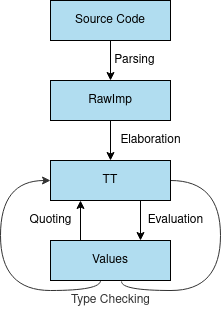
\includegraphics[scale=0.6]{./Resource/main.png}
\end{figure}
\end{multicols}
\end{frame}  

\begin{frame}[fragile]{Implementation}
  \begin{itemize}
    \item Language extended with holes `?hole\_name'.
    \item Synthesise individual terms or full pattern matching definitons.
    \item Repl extended with `auto' command for interaction.
    \item Testing functionality using pre-defined answer files and `t, test' commands.
    \item Attempts full context enumeration unlike other dependently typed systems.
  \end{itemize}
\end{frame}

\begin{frame}[fragile]{Term Synthesis}
\begin{multicols}{2}
  \begin{itemize}
  \item Local environment is searched first.
  \item Data Constructors second.
  \item Finally function definitions.
  \item Arguments are synthesised in a depth first traversal.
  \item Returns a list of results to be ordered.
  \item Order of synthesis is a heuristic.
  \end{itemize}

  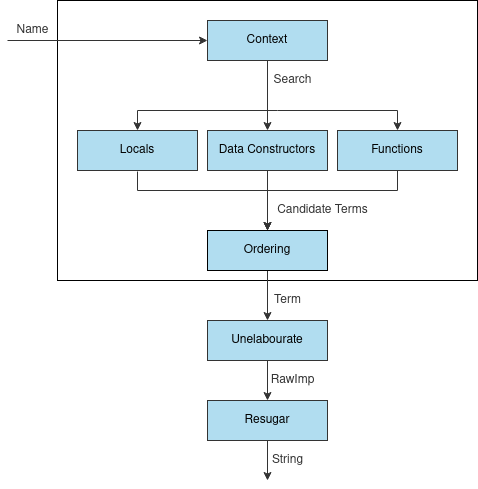
\includegraphics[scale=0.3]{Resource/syn.png}
  
\end{multicols}
\end{frame}

\begin{frame}[fragile]{Definition Synthesis}

\begin{multicols}{2}
  \begin{itemize}
  \item Given a type signature, construct a left hand side term to be split.
  \item Alternates between splitting on arguments and attempting synthesis. 
  \item Synthesis attempted for each left hand side.
  \item If all are successful the results are combined.
  \item If any fail the process attempts further splitting.
  \end{itemize}

  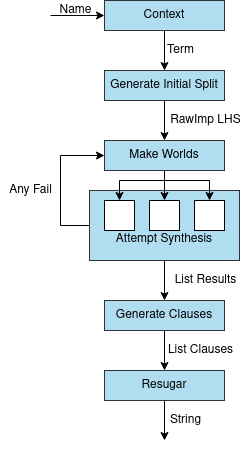
\includegraphics[scale=0.4]{Resource/worlds.png} 
\end{multicols}
\end{frame}

\begin{frame}[fragile]{Case Splitting} 
  \begin{itemize}
  \item An Initial split is performed on the leftmost type constructor.\\
  \item Splitting on all names that depend on the split argument is attempted. \\
  \item If the split results in only one case, new names are added and the process repeats until no names are left. \\ 
  \end{itemize}
  \begin{minted}[escapeinside=||]{idris}
    pat a : Type, |\colorbox{yellow}{n : Nat}|, m : Nat,
         |\colorbox{green}{xs : Vec n a}|, ys : Vec m a =>

   pat a : Type, m : Nat, ys : Vec m a =>
     append a Z m (Nil a) ys 
   pat a : Type, n : Nat, m : Nat, x : a, xs : Vec n a,
                                          ys : Vec m a =>
     append a (S n) m (Cons a n x xs) ys   
  \end{minted}
\end{frame}

\begin{frame}[fragile]{Case Splitting}
\begin{itemize}
\item LHS split into patterns before the split argument, and the scope.
\item Identify which patterns for the constructor have already been introduced.
\item Generate unique pattern variables for those which have not.
\item Replace references to the term with the application of the constructor.
\item Put the term back together and attempt to fill in any implicits generated. 
\end{itemize}
\begin{center}
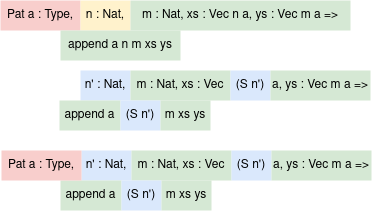
\includegraphics[scale=.5]{Resource/patSplit.png}
\end{center}
\end{frame}

\begin{frame}[fragile]{Evaluation}
  \begin{itemize}
  \item Tested with varying levels of type information.\\
  \item Compared to other similar systems.\\
  \item Idris, Idris2, Agda, Synquid.\\
  \item Evaluated based on the correctness of synthesised definitions.\\
  \item On each input returns the expected output.
  \end{itemize}
\end{frame}

\begin{frame}[fragile]{Evaluation - Lists}
\begin{center}
\begin{tabular}{|l|l|l|l|l|l|}
\hline
Problem & TinyIdris & Idris & Idris2 & Agda & Synquid \\
\hline
append &   &   & Pass &  &  \\
map &   &   & Pass &  & \\
replicate &   &   & Pass &  & \\
drop &   &   &   &  &   \\
foldr &   &   &   & &  \\
is empty &   &   &   &  & \\
is elem &   &   &   & &  \\
duplicate &   &   &   & &  \\
zip &   &   &   & & \\
i'th elem &   &   &   & & \\
index &   &   &   & & \\
\hline
\end{tabular}
\end{center}
\end{frame}

\begin{frame}[fragile]{Evaluation - Vectors}
\begin{center}
\begin{tabular}{|l|l|l|l|l|l|}
\hline
Problem & TinyIdris & Idris & Idris2 & Agda & Synquid \\
\hline
append & Pass & Pass & Pass & Pass & Pass\\
map & Pass  & Pass & Pass & Pass & Pass\\
replicate & Pass & Pass & &   & Pass\\
drop &   &   & Pass & Pass  & Pass\\
foldr &   &   &   &   & Pass\\
is empty &   &   &   &   & Pass\\
is elem &   &   &   &   & Pass\\
duplicate & Pass &   &   &   & Pass\\
zip &   & Pass & Pass & Pass  & Pass\\
i'th elem &   &   &   &   & Pass\\
index &   &   &   &   & Pass\\
\hline
\end{tabular}
\end{center}
\end{frame}

\begin{frame}[fragile]{Equalities}
  \begin{center}
\begin{tabular}{|l|l|l|l|l|l|}
\hline
Problem & TinyIdris & Idris & Idris2 & Agda & Synquid\\
\hline
andSymmetric & Pass & Pass & Pass & Pass & Pass \\
orSymmetric &  Pass & Pass & Pass & Pass & Pass \\
plus commutes &   &   &   & & - \\
plus Suc &   &   &   &  & - \\
symmetry &   & Pass & Pass & Pass & \\
transitivity &   & Pass & Pass & Pass & \\
congruence &   & Pass & Pass & Pass & - \\
list(vec(list)) = list &   & Pass & Pass & Pass & - \\
vec(list(list)) = vec &   &   & Pass &  & - \\
disjoint union apply &   &   &   & Pass & Pass \\
a = not not a &   &   &   &  & -\\
not not not a = not a &   &   & Pass & Pass & - \\
\hline
\end{tabular}
\end{center}
\end{frame}


\begin{frame}[fragile]{Heuristics}
\begin{center}
\begin{tabular}{|l|c|c|c|c|}
  
\hline
Problem & Loc-> DCon -> & Max Args & Rec + & Functions \\
 & Func & & Max Arg & Only \\
\hline
append & Pass & Pass & Pass & Pass\\
map & Pass  & & & Pass\\
replicate & Pass & & & Pass\\
drop &   & & & \\
foldr &   & & & \\
is empty &   & & & \\
is elem &   &  & & \\
duplicate & Pass & Pass & Pass & Pass\\
zip &   & & & \\
i'th elem &  & & & \\ 
index &   &  & & \\
\hline
\end{tabular}
\end{center}
\end{frame}


\begin{frame}[fragile]{Conclusions}
  \begin{itemize}
  \item Effectiveness limited due to the lack of constraint solving.\\
  \item Performance hindered by full enumeration.\\
  \item Heuristic less effective with full enumeration of the context.\\
  \item Prioritising language constructs that requires more built in knowledge may
    perform better than context enumeration.\\
  \item Type system extensions could provide more powerful definitions, as seen in Synquid.   
  \end{itemize}
\end{frame}


\end{document}
